% Options for packages loaded elsewhere
\PassOptionsToPackage{unicode}{hyperref}
\PassOptionsToPackage{hyphens}{url}
%
\documentclass[
  english,
  man]{apa6}
\usepackage{amsmath,amssymb}
\usepackage{lmodern}
\usepackage{ifxetex,ifluatex}
\ifnum 0\ifxetex 1\fi\ifluatex 1\fi=0 % if pdftex
  \usepackage[T1]{fontenc}
  \usepackage[utf8]{inputenc}
  \usepackage{textcomp} % provide euro and other symbols
\else % if luatex or xetex
  \usepackage{unicode-math}
  \defaultfontfeatures{Scale=MatchLowercase}
  \defaultfontfeatures[\rmfamily]{Ligatures=TeX,Scale=1}
\fi
% Use upquote if available, for straight quotes in verbatim environments
\IfFileExists{upquote.sty}{\usepackage{upquote}}{}
\IfFileExists{microtype.sty}{% use microtype if available
  \usepackage[]{microtype}
  \UseMicrotypeSet[protrusion]{basicmath} % disable protrusion for tt fonts
}{}
\makeatletter
\@ifundefined{KOMAClassName}{% if non-KOMA class
  \IfFileExists{parskip.sty}{%
    \usepackage{parskip}
  }{% else
    \setlength{\parindent}{0pt}
    \setlength{\parskip}{6pt plus 2pt minus 1pt}}
}{% if KOMA class
  \KOMAoptions{parskip=half}}
\makeatother
\usepackage{xcolor}
\IfFileExists{xurl.sty}{\usepackage{xurl}}{} % add URL line breaks if available
\IfFileExists{bookmark.sty}{\usepackage{bookmark}}{\usepackage{hyperref}}
\hypersetup{
  pdftitle={A Re-Analysis of Schroeder \& Epley (2015)},
  pdfauthor={Drew J. Shives1},
  pdflang={en-EN},
  pdfkeywords={re-analysis, reproducibility, communication, voice, speech, mind perception, social cognition, decision making, open data},
  hidelinks,
  pdfcreator={LaTeX via pandoc}}
\urlstyle{same} % disable monospaced font for URLs
\usepackage{graphicx}
\makeatletter
\def\maxwidth{\ifdim\Gin@nat@width>\linewidth\linewidth\else\Gin@nat@width\fi}
\def\maxheight{\ifdim\Gin@nat@height>\textheight\textheight\else\Gin@nat@height\fi}
\makeatother
% Scale images if necessary, so that they will not overflow the page
% margins by default, and it is still possible to overwrite the defaults
% using explicit options in \includegraphics[width, height, ...]{}
\setkeys{Gin}{width=\maxwidth,height=\maxheight,keepaspectratio}
% Set default figure placement to htbp
\makeatletter
\def\fps@figure{htbp}
\makeatother
\setlength{\emergencystretch}{3em} % prevent overfull lines
\providecommand{\tightlist}{%
  \setlength{\itemsep}{0pt}\setlength{\parskip}{0pt}}
\setcounter{secnumdepth}{-\maxdimen} % remove section numbering
% Make \paragraph and \subparagraph free-standing
\ifx\paragraph\undefined\else
  \let\oldparagraph\paragraph
  \renewcommand{\paragraph}[1]{\oldparagraph{#1}\mbox{}}
\fi
\ifx\subparagraph\undefined\else
  \let\oldsubparagraph\subparagraph
  \renewcommand{\subparagraph}[1]{\oldsubparagraph{#1}\mbox{}}
\fi
% Manuscript styling
\usepackage{upgreek}
\captionsetup{font=singlespacing,justification=justified}

% Table formatting
\usepackage{longtable}
\usepackage{lscape}
% \usepackage[counterclockwise]{rotating}   % Landscape page setup for large tables
\usepackage{multirow}		% Table styling
\usepackage{tabularx}		% Control Column width
\usepackage[flushleft]{threeparttable}	% Allows for three part tables with a specified notes section
\usepackage{threeparttablex}            % Lets threeparttable work with longtable

% Create new environments so endfloat can handle them
% \newenvironment{ltable}
%   {\begin{landscape}\centering\begin{threeparttable}}
%   {\end{threeparttable}\end{landscape}}
\newenvironment{lltable}{\begin{landscape}\centering\begin{ThreePartTable}}{\end{ThreePartTable}\end{landscape}}

% Enables adjusting longtable caption width to table width
% Solution found at http://golatex.de/longtable-mit-caption-so-breit-wie-die-tabelle-t15767.html
\makeatletter
\newcommand\LastLTentrywidth{1em}
\newlength\longtablewidth
\setlength{\longtablewidth}{1in}
\newcommand{\getlongtablewidth}{\begingroup \ifcsname LT@\roman{LT@tables}\endcsname \global\longtablewidth=0pt \renewcommand{\LT@entry}[2]{\global\advance\longtablewidth by ##2\relax\gdef\LastLTentrywidth{##2}}\@nameuse{LT@\roman{LT@tables}} \fi \endgroup}

% \setlength{\parindent}{0.5in}
% \setlength{\parskip}{0pt plus 0pt minus 0pt}

% \usepackage{etoolbox}
\makeatletter
\patchcmd{\HyOrg@maketitle}
  {\section{\normalfont\normalsize\abstractname}}
  {\section*{\normalfont\normalsize\abstractname}}
  {}{\typeout{Failed to patch abstract.}}
\patchcmd{\HyOrg@maketitle}
  {\section{\protect\normalfont{\@title}}}
  {\section*{\protect\normalfont{\@title}}}
  {}{\typeout{Failed to patch title.}}
\makeatother
\shorttitle{Schroeder \& Epley Re-Analysis}
\keywords{re-analysis, reproducibility, communication, voice, speech, mind perception, social cognition, decision making, open data}
\DeclareDelayedFloatFlavor{ThreePartTable}{table}
\DeclareDelayedFloatFlavor{lltable}{table}
\DeclareDelayedFloatFlavor*{longtable}{table}
\makeatletter
\renewcommand{\efloat@iwrite}[1]{\immediate\expandafter\protected@write\csname efloat@post#1\endcsname{}}
\makeatother
\usepackage{csquotes}
\ifxetex
  % Load polyglossia as late as possible: uses bidi with RTL langages (e.g. Hebrew, Arabic)
  \usepackage{polyglossia}
  \setmainlanguage[]{english}
\else
  \usepackage[main=english]{babel}
% get rid of language-specific shorthands (see #6817):
\let\LanguageShortHands\languageshorthands
\def\languageshorthands#1{}
\fi
\ifluatex
  \usepackage{selnolig}  % disable illegal ligatures
\fi
\newlength{\cslhangindent}
\setlength{\cslhangindent}{1.5em}
\newlength{\csllabelwidth}
\setlength{\csllabelwidth}{3em}
\newenvironment{CSLReferences}[2] % #1 hanging-ident, #2 entry spacing
 {% don't indent paragraphs
  \setlength{\parindent}{0pt}
  % turn on hanging indent if param 1 is 1
  \ifodd #1 \everypar{\setlength{\hangindent}{\cslhangindent}}\ignorespaces\fi
  % set entry spacing
  \ifnum #2 > 0
  \setlength{\parskip}{#2\baselineskip}
  \fi
 }%
 {}
\usepackage{calc}
\newcommand{\CSLBlock}[1]{#1\hfill\break}
\newcommand{\CSLLeftMargin}[1]{\parbox[t]{\csllabelwidth}{#1}}
\newcommand{\CSLRightInline}[1]{\parbox[t]{\linewidth - \csllabelwidth}{#1}\break}
\newcommand{\CSLIndent}[1]{\hspace{\cslhangindent}#1}

\title{A Re-Analysis of Schroeder \& Epley (2015)}
\author{Drew J. Shives\textsuperscript{1}}
\date{}


\authornote{

Drew J. Shives, Department of Psycholog, The Graduate Center of the City University of New York. Data from the orginal study used for this re-analysis can be found at \url{https://osf.io/nprmf/}

Correspondence concerning this article should be addressed to Drew J. Shives, 33-31 72nd Street, Jackson Heights, NY 11372. E-mail: \href{mailto:dshives@gradcenter.cuny.edu}{\nolinkurl{dshives@gradcenter.cuny.edu}}

}

\affiliation{\vspace{0.5cm}\textsuperscript{1} The Graduate Center of the City University of New York}

\abstract{
This re-analysis seeks to reproduce the results from Experiment \#1 of Schroeder and Epley (2015). In it, the authors sought to determine if listening, watching, or reading job candidates' pitches to hypothetical potential employers influenced how the candidates were evaluated. The subsequent evaluation was determined by three measures: candidates' perceived intellect, the general impression of the candidates, and the likelihood a candidate would be hired. Both Schroeder and Epley (2015) and the re-analysis found that there was a difference in all three measures between the audio and written conditions, but no difference between audio and video. Data from the orginal study used for this re-analysis can be found at \url{https://osf.io/nprmf/}
}



\begin{document}
\maketitle

\hypertarget{introduction}{%
\section{Introduction}\label{introduction}}

Schroeder and Epley (2015) hypothesized was that a person's speech conveys their fundamental capacity to think (reasoning, thoughtfulness, intellect, etc.) more clearly than the semantic content of just language alone. Similar to how variability of movement is an identifier of biological life, variability of voice may indicate a capable, lively mind. Therefore, a person should be viewed as having a greater mental capacity when an observer hears what they have to say rather than reading it.

To test this, M.B.A. students were asked to provide spoken and written pitches to hypothetical prospective employers. The spoken pitches were video recorded creating three experimental conditions --- audio, video, and written transcript. Each of the pitches for each condition (54 total) were evaluated by 3 individuals each. The evaluators were asked to assess the candidate's intellect, general impression, and likelihood of hiring based on the pitch. Schroeder and Epley (2015) believed that candidate would be viewed more positively (greater intellect, better general impression, and more hireable) if their pitch was listened to or watched rather than if it were only read.

\hypertarget{methods}{%
\section{Methods}\label{methods}}

\hypertarget{participants}{%
\subsection{Participants}\label{participants}}

18 M.B.A. students from the University of Chicago Booth School of Business were asked to provide the audio, video, and written transcripts of pitches to hypothetical prospective employers. They were provided a \$5 Starbucks giftcard for their participation. 162 individuals visiting the Museum of Science and Industry in Chicago were asked to review the candidates' pitches in exchange for a food item. Each of the pitches in each condition were reviewed by 3 evaluators (N = 54 per each condition).

\hypertarget{material}{%
\subsection{Material}\label{material}}

The M.B.A. students created pitches to hypothetical prospective employers which were video recorded. This created three separate experimental conditions --- audio, video, and written transcript.

\hypertarget{procedure}{%
\subsection{Procedure}\label{procedure}}

Upon listening, viewing, or reading a candidate's pitch, evaluators were asked to assess it across a variety of measures:

\begin{itemize}
\item
  Intellect: Evaluators were asked to answer 3 questions about the candidate's intellect --- (a) how competent the candidate seemed compared with the average candidate for an M.B.A. level position, (b) how thoughtful the candidate seemed compared with the average candidate for an M.B.A. level position, and (c) how intelligent the candidate compared with the average candidate for an M.B.A. level position. Each of these questions were answered on a scale of -5 to 5 (-5 = much less {[}competent, thoughtful, intelligent{]}, 5 = much more {[}competent, thoughtful, intelligent{]}) and then averaged with one another to create a composite measure of intellect.
\item
  Impression: Evaluators were asked to report their general impressions of the candidate --- (a) how much they liked the candidate, (b) how positive their overall impression of the candidate was, and (c) how negative their overall impression of the candidate was. Each of these was measured on a scale of 0 to 10 with 0 being the worst score and 10 being the best. These measures were then averaged with one another to form a composite measure of general impression.
\item
  Hire: Evaluators were asked to rate how likely they would be to hire the candidate (scale of 0 to 10 with 0 being the worst score and 10 being the best).
\end{itemize}

\hypertarget{data-analysis}{%
\subsection{Data analysis}\label{data-analysis}}

We used R {[}Version 4.1.1; R Core Team (2021){]} and the R-packages \emph{broom} {[}Version 0.7.10.9000; Robinson, Hayes, and Couch (2021){]}, \emph{dplyr} {[}Version 1.0.7; Wickham, François, Henry, and Müller (2021){]}, \emph{forcats} {[}Version 0.5.1; Wickham (2021a){]}, \emph{ggplot2} {[}Version 3.3.5; Wickham (2016){]}, \emph{haven} {[}Version 2.4.3; Wickham and Miller (2021){]}, \emph{lsr} {[}Version 0.5.2; Navarro (2015){]}, \emph{papaja} {[}Version 0.1.0.9997; Aust and Barth (2020){]}, \emph{purrr} {[}Version 0.3.4; Henry and Wickham (2020){]}, \emph{pwr} {[}Version 1.3.0; Champely (2020){]}, \emph{readr} {[}Version 2.0.2; Wickham and Hester (2021){]}, \emph{reshape2} {[}Version 1.4.4; Wickham (2007){]}, \emph{rstatix} {[}Version 0.7.0; Kassambara (2021){]}, \emph{schoRsch} {[}Version 1.9.1; Pfister and Janczyk (2020){]}, \emph{stringr} {[}Version 1.4.0; Wickham (2019){]}, \emph{tibble} {[}Version 3.1.5; Müller and Wickham (2021){]}, \emph{tidyr} {[}Version 1.1.4; Wickham (2021b){]}, \emph{tidyverse} {[}Version 1.3.1; Wickham et al. (2019){]}, and \emph{xtable} {[}Version 1.8.4; Dahl, Scott, Roosen, Magnusson, and Swinton (2019){]} for all our analyses.

Each of the experimental conditions (audio, video, written) were compared to one another for each measure (intellect, impression, hire) by several two independent sample t-tests and a one-way Analysis of Variance (ANOVA). Predictions made by the job candidates themselves were also analyzed, but are not included in this re-analysis.

\hypertarget{results}{%
\section{Results}\label{results}}

Overall mean and standard deviation results for each experimental condition and measure can be viewed in Table 1 and Figure 1.

Intellect for each job candidate in each Condition (Audio, Video, Written) was submitted to a one-way ANOVA.The main effect of Condition on Intellect was significant, \(F(2, 157) = 10.81\), \(\mathit{MSE} = 4.80\), \(p < .001\), \(\hat{\eta}^2_G = .121\).

Utilizing two independent sample t-tests, the audio condition was compared to the written and video conditions separately for intellect, impression, and hire.

Evaluators who heard pitches (M = 0.91, SD = 1.79) rather than reading them (M = -0.70, SD = 2.81) rated the candidates' intellect more highly, \(\Delta M = 1.61\), 95\% CI \([0.70\), \(2.51]\), \(t(105) = 3.52\), \(p = .001\). Evaluators who watched pitches (M = 1.09, SD = 1.80), however, did not evaluate candidates' intellect differently than evaluators who listened to pitches, \(\Delta M = -0.18\), 95\% CI \([-0.87\), \(0.51]\), \(t(104) = -0.51\), \(p = .608\).

Similarly, evaluators who heard pitches (M = 5.69, SD = 1.96) as opposed to reading them (M = 4.78, SD = 2.64) rated their impression of candidates more highly, \(\Delta M = 0.91\), 95\% CI \([0.02\), \(1.80]\), \(t(106) = 2.04\), \(p = .044\). Evaluators who watched pitches (M = 5.98, SD = 1.91) also did not differ in their impression of candidates from those who listened to their pitches, \(\Delta M = -0.28\), 95\% CI \([-1.02\), \(0.45]\), \(t(106) = -0.76\), \(p = .447\).

Likelihood to hire followed a similar pattern with evaluators who heard pitches (M = 4.34, SD = 2.26) more likely to hire candidates than those who read their pitches (M = 3.06, SD = 3.15), \(\Delta M = 1.28\), 95\% CI \([0.22\), \(2.34]\), \(t(103) = 2.40\), \(p = .018\). Evaluators who watched candidates' pitches (M = 4.46, SD = 2.43) were no more likely to hire a candidate than evaluators who heard the pitches, \(\Delta M = -0.12\), 95\% CI \([-1.02\), \(0.78]\), \(t(105) = -0.27\), \(p = .786\).

\hypertarget{simulation-based-power-analysis}{%
\section{Simulation-Based Power Analysis}\label{simulation-based-power-analysis}}

The design of Experiment \#1 centered around investigating whether hearing (or seeing) versus reading a candidate's pitch would change evaluators' perception of them in terms of intellect, general impression, and hireability. Each experimental condition (audio, video, and written) had 54 evaluations (N = 54). The focus of this simulation-based power analysis will be on intellect and at what effect size will there be a determinable difference from the written condition.

Power represents the probability that an experimental design will reject the null-hypothesis given that there is a true effect. Power is thus dependent on the size of that true effect --- a design will have greater power to detect a large difference versus a small one. Cohen's D, a mean difference in terms of standard deviation units, is a commonly used measure to define the true difference between treatments. (Power is also dependent on sample-size and alpha-criterion.)

To begin, the overall mean score for intellect and the standard deviation of the mean intellect score are calculated for the written condition (-0.70 and 2.81, respectively). Our goal is to determine how large of an effect size is needed to produce an ascertainable difference from the written condition.

Using the rnorm function to generate simulated data for each subject, we model the effect of listening (or watching) to a candidate's pitch by increasing the mean in this condition by a proportion of the standard deviation. This proportion is determined by effect size; we used effect sizes ranging from 0.1 to 1.0. For each effect size, we run 1000 simulated experiments and save the p-value for the effect of the audio condition for each simulation. For each effect size, we then find the proportion of experimental simulations that had a p-value less than 0.5 as the proportion of experiments where the null can be rejected is the power of the design to detect an effect of each effect size.

The below simulation finds that this design had a power of 0.75 to detect an effect of d = 0.5. It had power of 0.98 to detect effects of d = 0.8. The full results and power curve can be viewed in Table 2 and Figure 2, respectively.

While the actual power of listening vs.~reading for intellect is quite high (d = 0.68), it can be improved by increasing the amount of evaluators per condition, increasing the alpha parameter, or increasing the actual effect size.

\hypertarget{discussion}{%
\section{Discussion}\label{discussion}}

The re-analysis, unfortunately, did not reproduce the analysis reported by Schroeder and Epley (2015). This was mainly due to the authors reporting incorrect t-tests for Experiment \#1. This can be inferred from the degrees of freedom reported for each test. For example, when comparing intellect between evaluators who listened to pitches and those who read them, the authors reported a degrees of freedom for their t-test as 157. This is impossible as the total number of evaluators per experimental condition (before attributing to any NAs in the data) is 54, meaning that the total amount of evaluators to be considered when calculating the degrees of freedom for the t-test is 108.

Even still, the re-analysis was able to reproduce the general findings of Schroeder and Epley (2015) if not the exact numbers.

\begin{table}[tbp]

\begin{center}
\begin{threeparttable}

\caption{\label{tab:table}Means and Standard Deviations of Measures by Condition}

\begin{tabular}{llllllll}
\toprule
Condition & \multicolumn{1}{c}{n} & \multicolumn{1}{c}{Mean Intel.} & \multicolumn{1}{c}{SD Intel.} & \multicolumn{1}{c}{Mean Impr.} & \multicolumn{1}{c}{SD Impr.} & \multicolumn{1}{c}{Mean Hire} & \multicolumn{1}{c}{SD Hire}\\
\midrule
audio & 54 & 0.91 & 1.79 & 5.69 & 1.96 & 4.34 & 2.26\\
transcript & 54 & -0.70 & 2.81 & 4.78 & 2.64 & 3.06 & 3.15\\
video & 54 & 1.09 & 1.80 & 5.98 & 1.91 & 4.46 & 2.43\\
\bottomrule
\end{tabular}

\end{threeparttable}
\end{center}

\end{table}

\begin{figure}
\centering
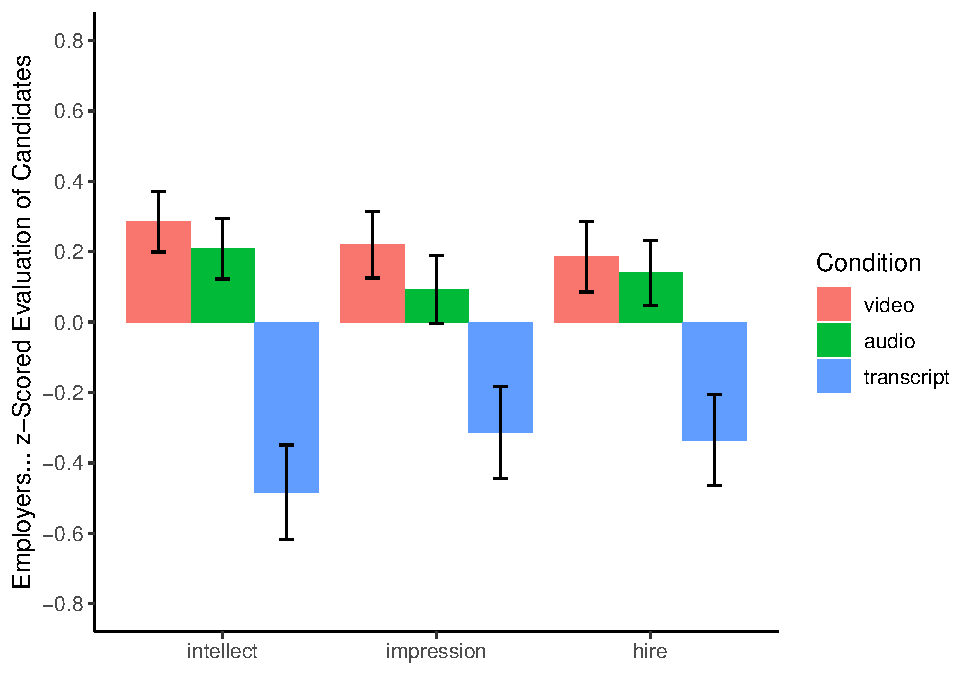
\includegraphics{APA_report_files/figure-latex/unnamed-chunk-15-1.pdf}
\caption{\label{fig:unnamed-chunk-15}Results from Experiment \#1. Evaluators' standardized ratings of the job candidates' intellect, their general impressions of the candidates, and their likelihood of hiring the candidates. Results are shown separately for the video, audio, and transcript conditions. Error bars represent +1 and -1 SEM.}
\end{figure}

\begin{table}[tbp]

\begin{center}
\begin{threeparttable}

\caption{\label{tab:unnamed-chunk-16}Results from the simulation-based power analysis.}

\begin{tabular}{ll}
\toprule
effect\_sizes & \multicolumn{1}{c}{power}\\
\midrule
0.10 & 0.07\\
0.15 & 0.13\\
0.20 & 0.18\\
0.25 & 0.26\\
0.30 & 0.33\\
0.35 & 0.43\\
0.40 & 0.54\\
0.45 & 0.67\\
0.50 & 0.72\\
0.55 & 0.83\\
0.60 & 0.87\\
0.65 & 0.91\\
0.70 & 0.94\\
0.75 & 0.97\\
0.80 & 0.98\\
0.85 & 1.00\\
0.90 & 1.00\\
0.95 & 1.00\\
1.00 & 1.00\\
\bottomrule
\end{tabular}

\end{threeparttable}
\end{center}

\end{table}

\begin{figure}
\centering
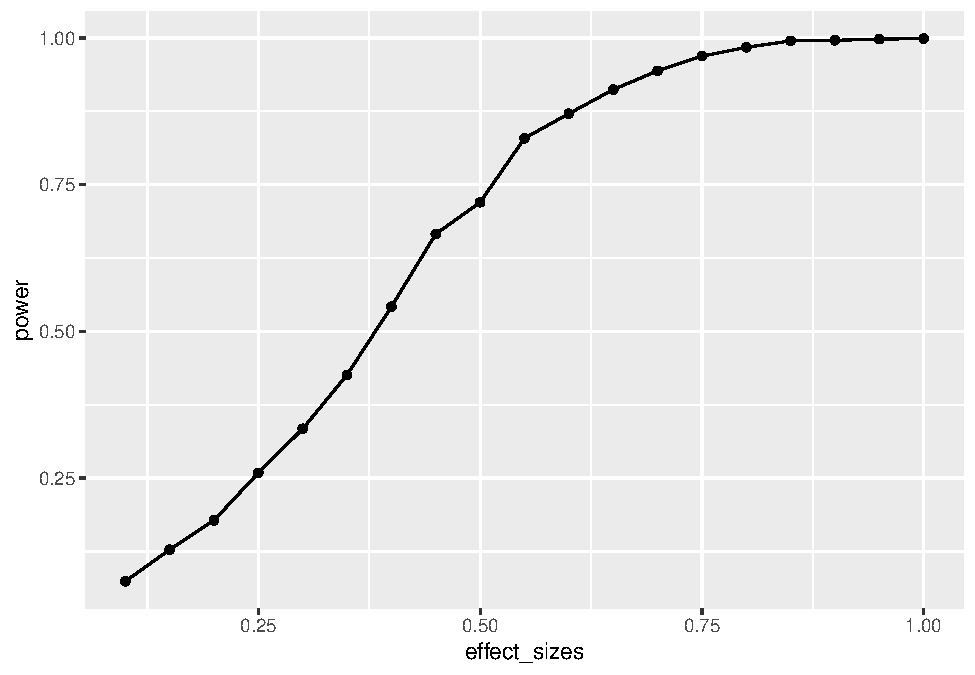
\includegraphics{APA_report_files/figure-latex/unnamed-chunk-17-1.pdf}
\caption{\label{fig:unnamed-chunk-17}Simulation-based power curve for this design.}
\end{figure}

\newpage

\hypertarget{references}{%
\section{References}\label{references}}

\begingroup
\setlength{\parindent}{-0.5in}
\setlength{\leftskip}{0.5in}

\hypertarget{refs}{}
\begin{CSLReferences}{1}{0}
\leavevmode\hypertarget{ref-R-papaja}{}%
Aust, F., \& Barth, M. (2020). \emph{{papaja}: {Create} {APA} manuscripts with {R Markdown}}. Retrieved from \url{https://github.com/crsh/papaja}

\leavevmode\hypertarget{ref-R-pwr}{}%
Champely, S. (2020). \emph{Pwr: Basic functions for power analysis}. Retrieved from \url{https://CRAN.R-project.org/package=pwr}

\leavevmode\hypertarget{ref-R-xtable}{}%
Dahl, D. B., Scott, D., Roosen, C., Magnusson, A., \& Swinton, J. (2019). \emph{Xtable: Export tables to LaTeX or HTML}. Retrieved from \url{https://CRAN.R-project.org/package=xtable}

\leavevmode\hypertarget{ref-R-purrr}{}%
Henry, L., \& Wickham, H. (2020). \emph{Purrr: Functional programming tools}. Retrieved from \url{https://CRAN.R-project.org/package=purrr}

\leavevmode\hypertarget{ref-R-rstatix}{}%
Kassambara, A. (2021). \emph{Rstatix: Pipe-friendly framework for basic statistical tests}. Retrieved from \url{https://CRAN.R-project.org/package=rstatix}

\leavevmode\hypertarget{ref-R-tibble}{}%
Müller, K., \& Wickham, H. (2021). \emph{Tibble: Simple data frames}. Retrieved from \url{https://CRAN.R-project.org/package=tibble}

\leavevmode\hypertarget{ref-R-lsr}{}%
Navarro, D. (2015). \emph{Learning statistics with r: A tutorial for psychology students and other beginners. (Version 0.6)}. Sydney, Australia: University of New South Wales. Retrieved from \url{https://learningstatisticswithr.com}

\leavevmode\hypertarget{ref-R-schoRsch}{}%
Pfister, R., \& Janczyk, M. (2020). \emph{schoRsch: Tools for analyzing factorial experiments}. Retrieved from \url{https://CRAN.R-project.org/package=schoRsch}

\leavevmode\hypertarget{ref-R-base}{}%
R Core Team. (2021). \emph{R: A language and environment for statistical computing}. Vienna, Austria: R Foundation for Statistical Computing. Retrieved from \url{https://www.R-project.org/}

\leavevmode\hypertarget{ref-R-broom}{}%
Robinson, D., Hayes, A., \& Couch, S. (2021). \emph{Broom: Convert statistical objects into tidy tibbles}.

\leavevmode\hypertarget{ref-R-reshape2}{}%
Wickham, H. (2007). Reshaping data with the {reshape} package. \emph{Journal of Statistical Software}, \emph{21}(12), 1--20. Retrieved from \url{http://www.jstatsoft.org/v21/i12/}

\leavevmode\hypertarget{ref-R-ggplot2}{}%
Wickham, H. (2016). \emph{ggplot2: Elegant graphics for data analysis}. Springer-Verlag New York. Retrieved from \url{https://ggplot2.tidyverse.org}

\leavevmode\hypertarget{ref-R-stringr}{}%
Wickham, H. (2019). \emph{Stringr: Simple, consistent wrappers for common string operations}. Retrieved from \url{https://CRAN.R-project.org/package=stringr}

\leavevmode\hypertarget{ref-R-forcats}{}%
Wickham, H. (2021a). \emph{Forcats: Tools for working with categorical variables (factors)}. Retrieved from \url{https://CRAN.R-project.org/package=forcats}

\leavevmode\hypertarget{ref-R-tidyr}{}%
Wickham, H. (2021b). \emph{Tidyr: Tidy messy data}. Retrieved from \url{https://CRAN.R-project.org/package=tidyr}

\leavevmode\hypertarget{ref-R-tidyverse}{}%
Wickham, H., Averick, M., Bryan, J., Chang, W., McGowan, L. D., François, R., \ldots{} Yutani, H. (2019). Welcome to the {tidyverse}. \emph{Journal of Open Source Software}, \emph{4}(43), 1686. \url{https://doi.org/10.21105/joss.01686}

\leavevmode\hypertarget{ref-R-dplyr}{}%
Wickham, H., François, R., Henry, L., \& Müller, K. (2021). \emph{Dplyr: A grammar of data manipulation}. Retrieved from \url{https://CRAN.R-project.org/package=dplyr}

\leavevmode\hypertarget{ref-R-readr}{}%
Wickham, H., \& Hester, J. (2021). \emph{Readr: Read rectangular text data}. Retrieved from \url{https://CRAN.R-project.org/package=readr}

\leavevmode\hypertarget{ref-R-haven}{}%
Wickham, H., \& Miller, E. (2021). \emph{Haven: Import and export 'SPSS', 'stata' and 'SAS' files}. Retrieved from \url{https://CRAN.R-project.org/package=haven}

\end{CSLReferences}

\endgroup


\end{document}
